\section{Zielsetzung}

Der Versuch V$\num{401}$ setzt sich in erster Linie mit dem Michelson--Interferrometer
auseinander. Die Wellenlänge der verwendeten Lichtquelle, wowie der Brechungsindex
verschiedener Gase sollen im Laufe des Versuches bestimmt werden.

\section{Theorie}

Das Michelson-Interferometer ist ein Messgerät, welches auf dem Interferenzprinzip
beruht. Das Ausbreitungsverhalten von Licht kann sehr gut durch das
Verhalten von elektromagnetischen Wellen beschrieben werden.
Da die Maxwellschen-Gleichungen durch lineare Differentialgleichungen gegeben sind,
können ihre Lösungen, welche auch elektromagnetische Wellen sind, superponiert werden.
Der $\vec{E}$-Feld Vektor kann jedoch nicht direkt bestimmt werden, sondern
lediglich seine Intensität, die gegeben ist durch

\begin{equation}
  \label{eqn:Intensitaet}
  I = \left|\vec{E}\right|^2.
\end{equation}

Aus der Superposition zweier Wellen mit verschiedenen Phasen ($\delta_1, \delta_2$)
entsteht neben der Summe der Einzelintensitäten noch ein Interfenezterm,
der das Verhalten der Überlagerung der beiden Wellen beschreibt.
Dieser Term weist die folgende Gestalt auf.

\begin{align}
  \label{eqn:Interferenterm}
  &2k\vec{E}_0^2\cos{(\delta_2 - \delta_1)},& k\in \mathbb{R}
\end{align}

Da der Kosinus beschränkt ist, ist auch der Interferenzterm beschränkt
durch $\pm 2k\vec{E}_0$. Wenn das Argument ein Vielfaches von
$\frac{n\pi}{2} + \pi$ mit $n\in \mathbb{N}$ ist verschwindet der
Interferenzterm.

Bei den alltäglichen Lichtquellen treten keine Interferenzeffekte auf,
da die Phasenbeziehungen $\delta_i$ normalerweise Funktionen der Zeit sind.
Dies ist auf den statistischen Prozesses der Lichterzeugung zurückzuführen.
Licht, dessen Phasenbeziehung nicht konstant ist wird als inkohärent bezeichnet.

Damit Interferenzeffekte auftreten muss die Phasenbeziehung unabhängig
von der Zeit $t$ sein. Solch ein Licht wird als kohärent bezeichnet.

Nur Licht aus der selben Quelle weist die gleiche Phasenbeziehnung auf. Damit
dies möglich ist, wird ein Strahlteiler verwendet. Die geteilten Strahlen
legen im Allgemeinen unterschiedliche Strecken zurück, weshalb sie
eine Phasenverschiebung zueinander aufweisen.
Der Emmissionsakt aus der Lichtquelle ist ein endlicher Prozess, dessen
Zeitdauer als Kohärenzzeit $\tau$ bezeichnet wird. Ist die Kohärenzzeit
kleiner klein gegenüber $\propto \lambda$ verschwinden die Interferenzeffekte,
da aufgrund der endlichen Lichtgeschwindigkeit Licht aus verschiedenen
Quellen an dem Detektor registriert wird.
Daraus folgt, dass eine notwendige Bedingung für das Erscheinen von
Interferenzeffekten, ein geringer Wegunterschied zwischen den geteilten
Strahlen ist. Der Wegunterschied, bei dem die Interferenzeffekte verschwinden
wird als Kohärenzlänge $\ell$ bezeichnet. Diese wird charakterisiert über

\begin{equation}
  \label{eqn:Kohärenzlänge}
  \ell = \symup{N}\lambda,\;\text{(N: Anzahl der am Detektor beobachteten Intensitätsmaxima)}.
\end{equation}

Die Kohärenzzeit hängt mit der Kohärenzlänge eng zusammen.
Die beiden Größen sind über den folgenden Zusammenhang \eqref{eqn:Kohärenz} erklärt.

\begin{equation}
  \label{eqn:Kohärenz}
  \tau = \frac{\ell}{c}
\end{equation}

Die verwendete Lichtquelle sollte möglichst als punktförmig approximiert werden können,
da ansonsten der Kontrast des Interferenzmusters verschlechter wird.
Als angemessene Forderung die Ungleichung \eqref{eqn:Kohärenzbed}.

\begin{equation}
  \label{eqn:Kohärenzbed}
  a \sin{(\zeta)} << \frac{\lambda}{2}
\end{equation}

In \eqref{eqn:Kohärenzbed} ist $a$ die räumliche Ausdehnung der Lichtquelle und
$\zeta$ der Richtungsunterschied. Die Größen sind in Abb. \ref{fig:ausgedehnte_Quelle}
abgebildet.

\begin{figure}
  \centering
  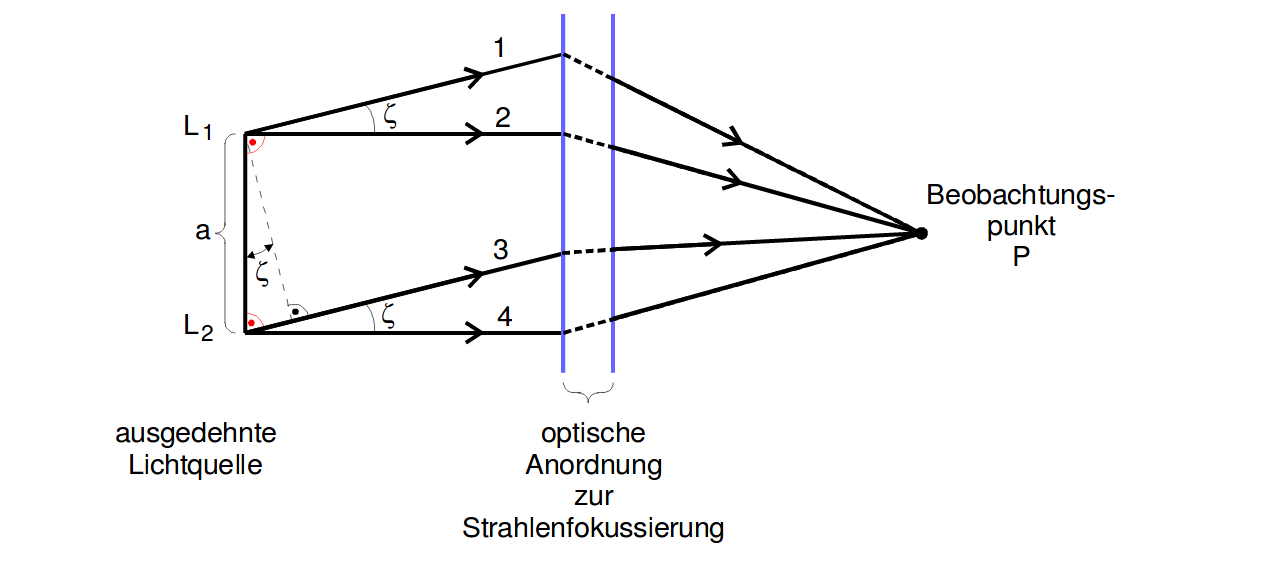
\includegraphics[width=\textwidth]{ausgedehnte_Quelle.png}
  \caption{Darstellung der Winkelbeziehungen einer ausgedehnten Lichtquelle\cite{sample}}
  \label{fig:ausgedehnte_Quelle}
\end{figure}

Die Bedingung \eqref{eqn:Kohärenzbed} lässt sich aus der Vorderung folgern, dass
das ausgesendete Licht in dem Punkt P interferenzfähig ist.


\section{Durchführung}

Der Versuch ist mit der in Abb.\ref{fig:Apparatur} durchzuführen.
Die Lichtquelle ist ein Laser, der kohärentes Licht gewährleistet.
Eine konstante Phasenbeziehung zwischen den interferierenden Lichtstrahlen ist
durch den Strahlteiler gegeben. Die geteilten Strahlen entstammen der selben Quelle
und haben somit eine zueinander konstante Phasenbeziehnung.
Die Messzelle kann mit Gasen befüllt werden und dient zur Bestimmung
des Brechungsindex des Füllgases. Die Messzelle ist mit einer Vakuumpumpe und einer
Gasflasche über Schlauchsysteme verbunden.
Der justierbare Spiegel ist notwendig
fpr die Kalibrierung der Apparatur. Der Synchromotor verstellt den
verschiebaren Spiegel, sodass die Weglänge und somit die Phasenverschiebung
zwischen den geteilten Strahlen präzise und kontinuierlich verändert werden kann.
Als Detektor fungiert ein Photoelement, dass die veränderlichen Intensitätsmaxima
registriert und über eine Zählwerk abzählbar darstellt.

\begin{figure}
  \centering
  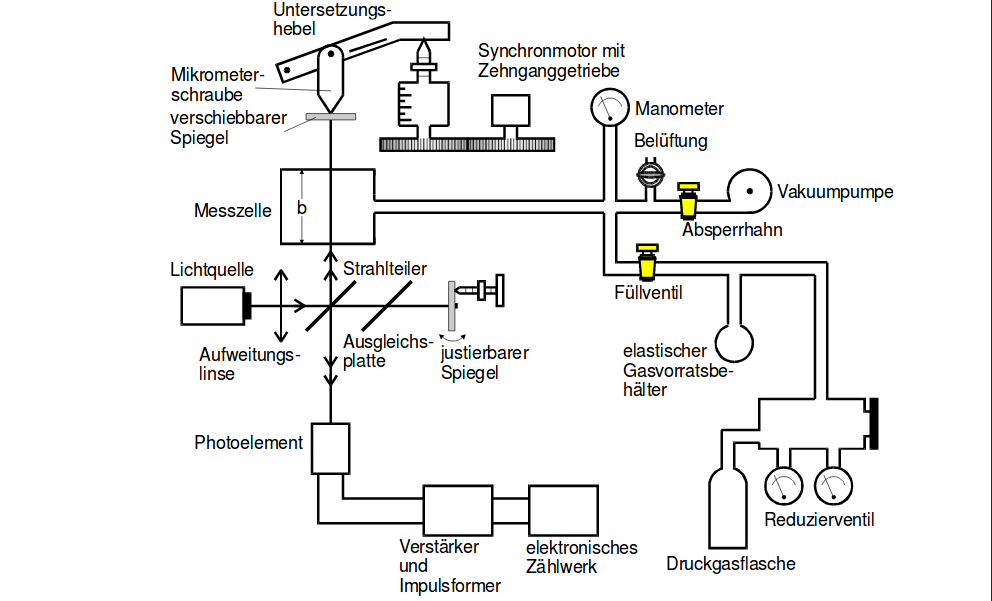
\includegraphics[width=\textwidth]{Interferometer.png}
  \caption{Schematische Darstellung der verwendeten Apparatur\cite{sample}}
  \label{fig:Apparatur}
\end{figure}

Zu Beginn des Versuches ist die Apparatur zu kalibrieren. Dabei kann eine
Mattscheibe, oder ein Blattpapier verwendet werden, um die Inteferenzmaxima
sichtbar zu machen. Über eine Schraube an dem justierbaren Spiegel wird die Apparatur kalibriert.
Die Kalibrierung ist abgeschlossen, wenn die beiden geteilten
Strahlen auf dem Detektor zusammen geführt sind und ein Inteferenzmuster ausbilden.
Je gröber das Interferenzmuster ist, desto besser, weil das Zählwerk die
auftretende Maximafluktiation zuverlässiger zählen kann.

Für die erste Messung wird zuerst die Startposition des Motors notiert.
Dieser wird danach angeschaltet und während dieser läuft zählt das Zählwerk
die auftretenden Intensitätsmaxima. Die Messung ist abgeschlossen, wenn $\approx 1000$
Werte genommen sind. Abschließend ist die Endposition des Motors an der Millimeterschraube
abzulesen. Der Messvorgang wird zehn mal widerholt.
Durch die erste Messung ist die Wellenlänge der verwendeten Lichtquelle zu bestimmen.

Die zweite Messung zielt darauf ab, die Brechungsindizes verschiedener Gase
zu ermitteln. Als erstes wird der Brechungsindex von Luft ermittelt.
Dafür wird die Messzelle, die in Abb. \ref{fig:Apparatur} dargestellt ist evakuiert.
Bei ausreichender Evakuierung wird eine Stellschraube an der Vakuumpumpe gelockert,
sodass Luft in die Messzelle eindringen kann. Die Druckdifferenz, sowie die
abgezählten Intensitätsmaxima sind zu notieren.
Die Messung wird zehn mal widerholt und daraufhin mit $\ce{CO_2}$ widerholt.
Dafür ist eine $\ce{CO_2}$-Flasche an die Messzelle angeschlossen.
Nach Evakuierung der Zelle kann so das Gas in diese eingefüllt werden.
Auch hier sind zehn Messungen durchzuführen.
